\documentclass{beamer}
\mode<presentation>
\usepackage{amsmath}
\usepackage{amssymb}
%\usepackage{advdate}
\usepackage{graphicx}
\graphicspath{{../figs/}}
\usepackage{adjustbox}
\usepackage{subcaption}
\usepackage{enumitem}
\usepackage{multicol}
\usepackage{mathtools}
\usepackage{listings}
\usepackage{url}
\def\UrlBreaks{\do\/\do-}
\usetheme{Boadilla}
\usecolortheme{lily}
\setbeamertemplate{footline}
{
  \leavevmode%
  \hbox{%
  \begin{beamercolorbox}[wd=\paperwidth,ht=2.25ex,dp=1ex,right]{author in head/foot}%
    \insertframenumber{} / \inserttotalframenumber\hspace*{2ex} 
  \end{beamercolorbox}}%
  \vskip0pt%
}
\setbeamertemplate{navigation symbols}{}
\let\solution\relax
\usepackage{gvv}
\lstset{
%language=C,
frame=single, 
breaklines=true,
columns=fullflexible
}

\numberwithin{equation}{section}



\begin{document}

\title{4.10.22}
\author{EE25BTECH11020 - Darsh Pankaj Gajare}
% \maketitle
% \newpage
% \bigskip
%\begin{document}
{\let\newpage\relax\maketitle}
%\renewcommand{\thefigure}{\theenumi}
%\renewcommand{\thetable}{\theenumi}
Question:\\
Find the equation of the plane through the intersection of the planes $\vec{r}\cdot\brak{\hat{i}+3\hat{j}}-6=0$ and $\vec{r}\cdot\brak{3\hat{i}-\hat{j}-4\hat{k}}=0$,whose perpendicular distance from origin is unity.\\
\solution
\begin{table}[H]
	\centering
	\caption{}
	\begin{tabular}{|c|c|}
\hline
\textbf{Name} & \textbf{Value} \\ \hline
$\vec{A}$ & $\myvec{2 & 1 \\0 & 3}$ \\ \hline
\end{tabular}

	\label{}
\end{table}
\solution
The given planes are
\begin{align}
\vec{x}^\top\vec{n}_1 - 6 = 0 \\
\vec{x}^\top\vec{n}_2 = 0
\end{align}
Let the required plane be
\begin{align}
\vec{x}^\top\brak{\vec{n}_1 + \lambda\vec{n}_2} - 6 = 0
\end{align}
the normal vector is
\begin{align}
\vec{n} = \vec{n}_1 + \lambda\vec{n}_2
\end{align}
\begin{align}
\norm{\vec{n}}^2 = \vec{n}^\top\vec{n}= \vec{n}_1^\top\vec{n}_1 + 2\lambda\vec{n}_1^\top\vec{n}_2 + \lambda^2 \vec{n}_2^\top\vec{n}_2
\end{align}
Perpendicular distance from origin is
\begin{align}
\frac{\abs{-6}}{\norm{\vec{n}}} &= 1 \\
\norm{\vec{n}} = 6
\end{align}
Hence,
\begin{align}
\vec{n}_1^\top\vec{n}_1 + 2\lambda\vec{n}_1^\top\vec{n}_2 + \lambda^2 \vec{n}_2^\top\vec{n}_2 = 36
\end{align}
\begin{align}
10 + 26\lambda^2 = 36 \\
\lambda = \pm 1
\end{align}
Thus, the required planes are
\begin{align}
	\myvec{2\\1\\-2}^\top\vec{x}=3\\
	\myvec{1\\-2\\-2}^\top\vec{x}=-3
\end{align}

\begin{figure}[H]
	\centering
	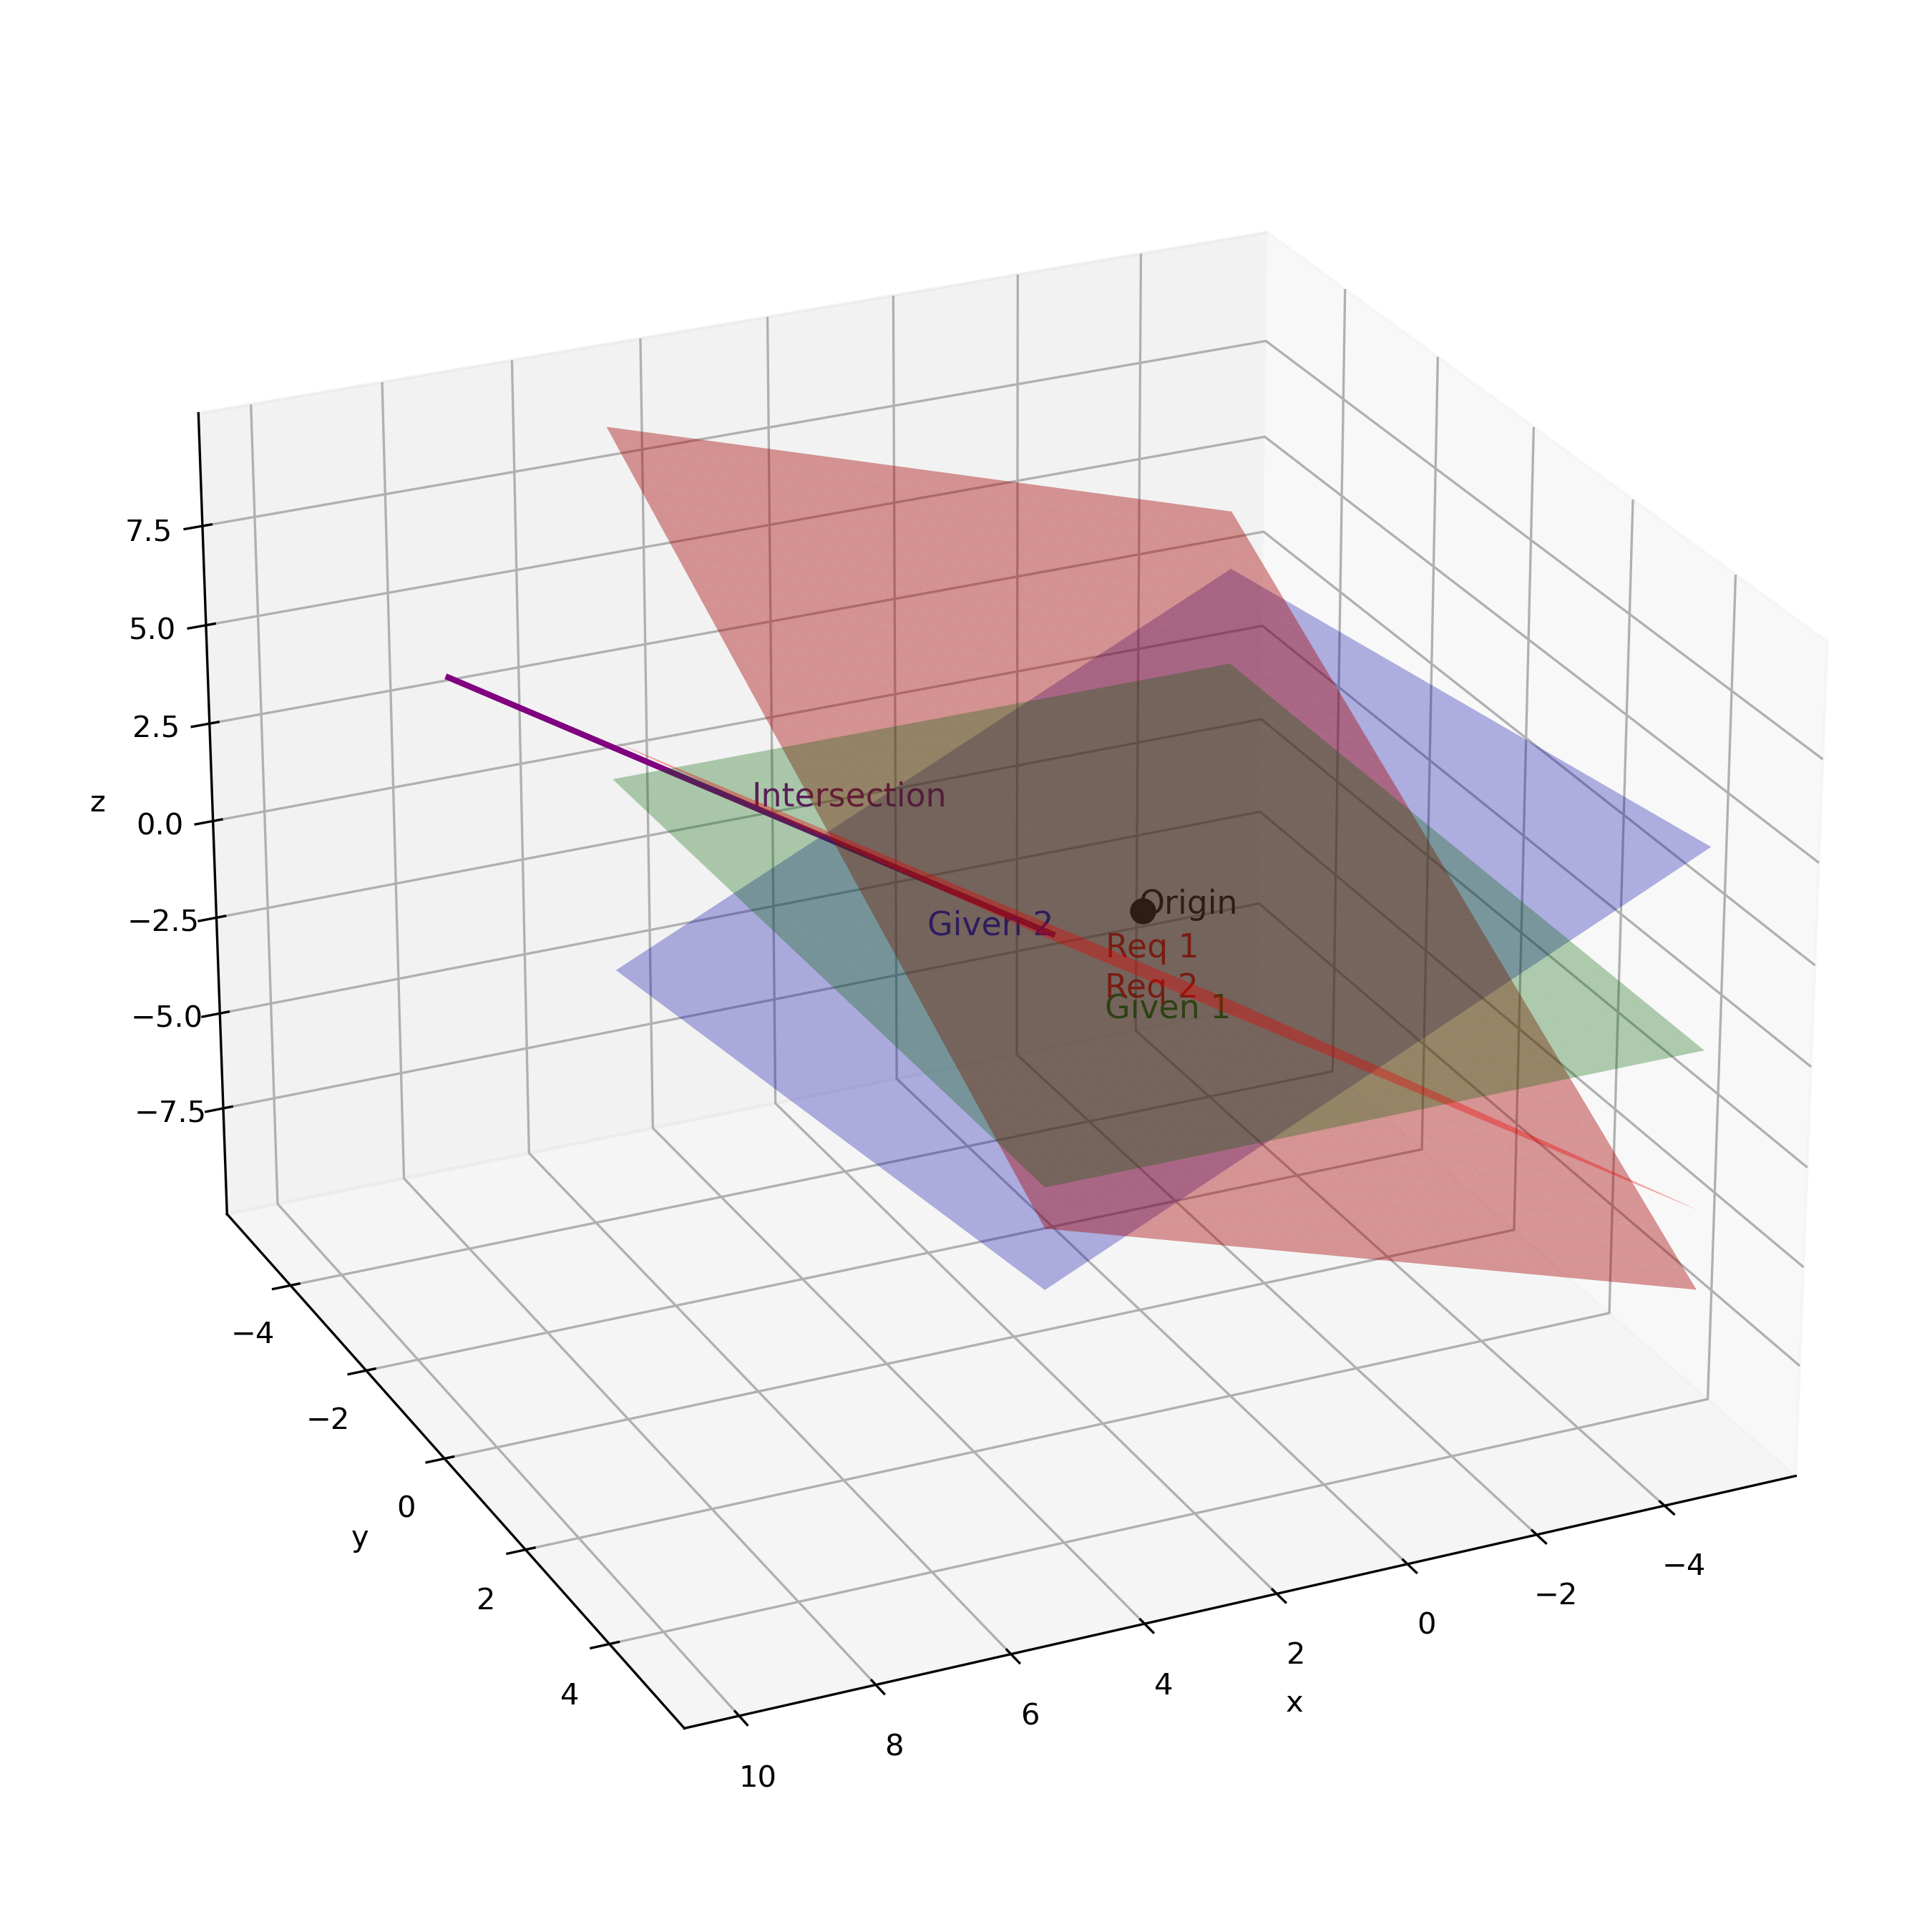
\includegraphics[scale=0.25]{img1}
	\caption*{Plot using C libraries}
	\label{img1}
\end{figure}
\begin{figure}[H]
	\centering
	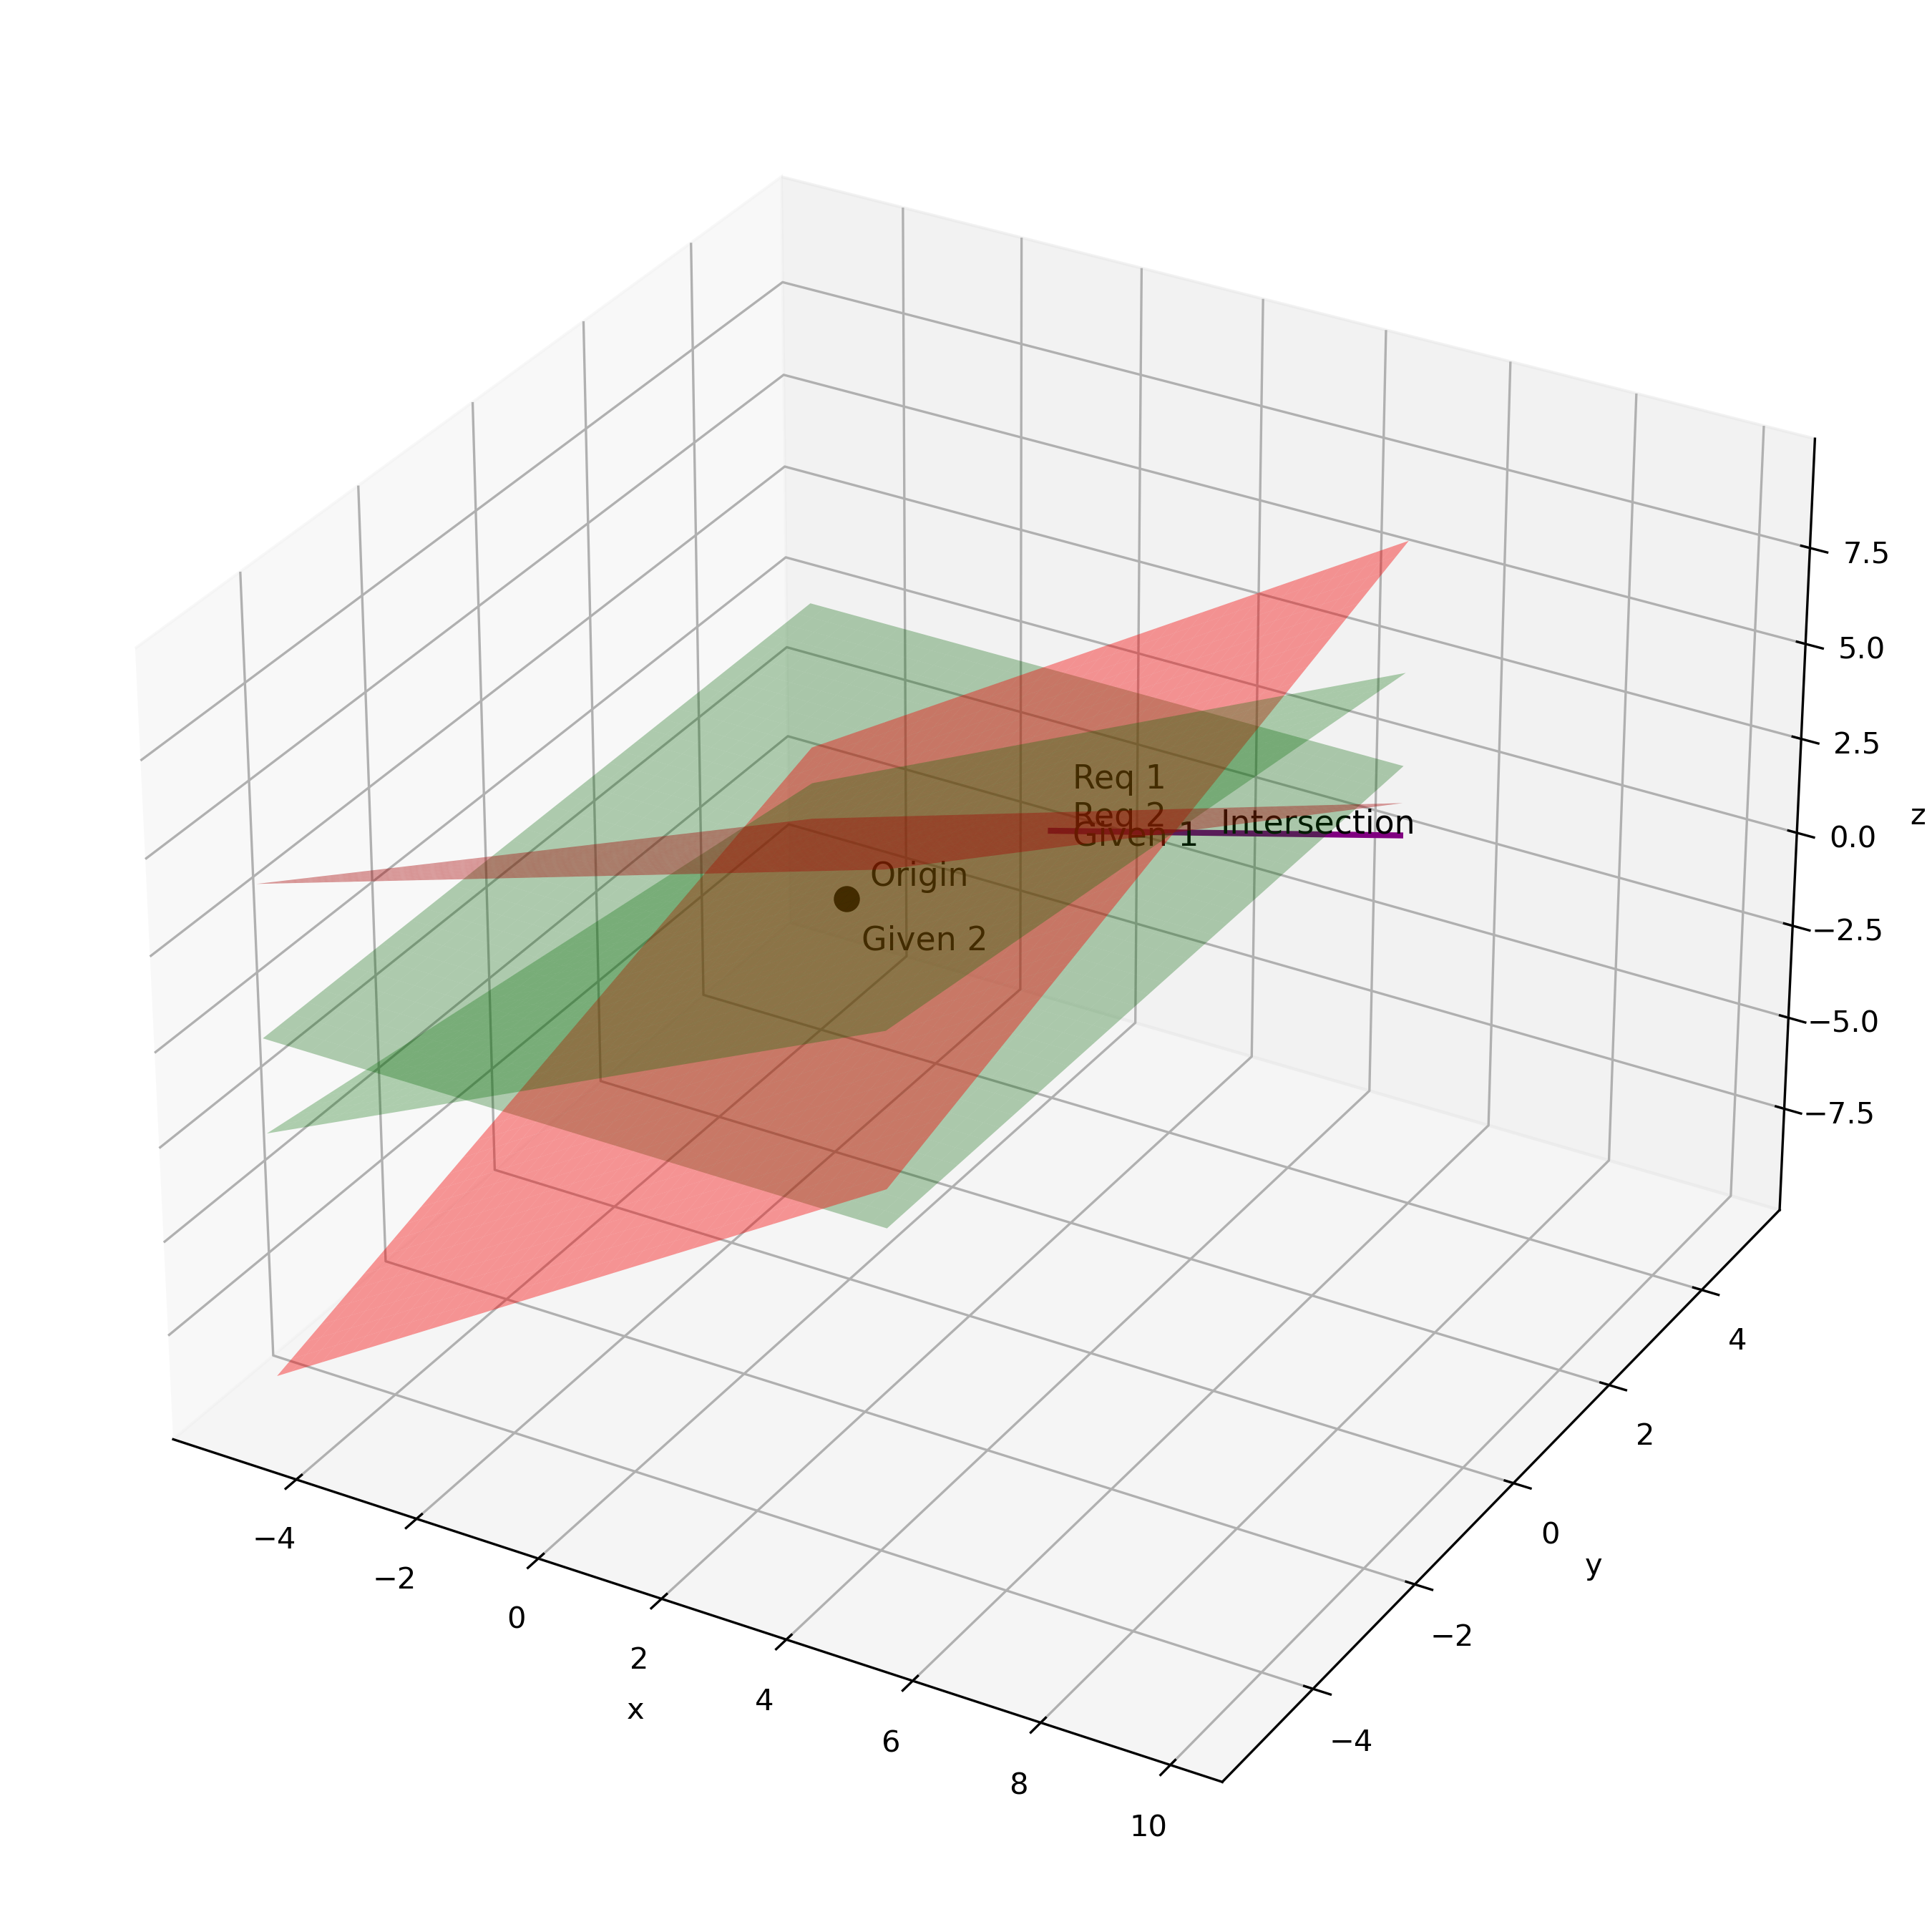
\includegraphics[scale=0.25]{img2}
	\caption*{Plot using Python}
	\label{img2}
\end{figure}
\end{document}

